
\documentclass[a4paper,11pt]{article}
\usepackage[T1]{fontenc}
\usepackage[italian,english]{babel}
\usepackage[utf8]{inputenc}
\usepackage[xindy]{imakeidx}
\usepackage{xcolor}
\usepackage{graphicx}
\usepackage{amsmath}
\usepackage{amssymb}
\usepackage{etaremune}
\usepackage{enumitem}
\usepackage[toc,page]{appendix}
\usepackage{verbatimbox}
\usepackage{tabularx}
\usepackage{booktabs}
% \usepackage{wrapfig} % immagini avvolte dal testo

\usepackage[hidelinks, colorlinks=true, linkcolor=black, urlcolor=blue]{hyperref}	
\usepackage{bookmark}
\usepackage{caption}
\usepackage{subfig}

\captionsetup{tableposition=top, figureposition=bottom, font=small}
\setcounter{tocdepth}{3}
\setcounter{secnumdepth}{3}

\usepackage{epigraph}


\makeindex


\includeonly{
			sections/AnalisiPreliminare,%
			sections/AssiDiComunicazione,%
			sections/Contenuto,%
			sections/Pubblicita,%
			sections/Ricerca,%
			sections/Mobile,%
			sections/Conclusioni%
			}
		
\begin{document}

\title{Analisi di usabilità}
\author{Eduard Bicego}
\date{}

\maketitle

%



\begin{table} [h]
		\centering
		\begin{tabular}{c|c}
			%\toprule
			Sito analizzato & \href{http://www.cinisio.com/}{www.cinisio.com} \\
			\midrule
			Periodo analisi & Maggio/Giugno 2016 \\
			%\bottomrule
		\end{tabular}
	
\end{table}


\begin{abstract}

	Il presente documento si propone di discutere e mettere in evidenza le problematiche dell'usabilità rilevate durante l'analisi del sito web \href{http://www.cinisio.com/}{www.cinisio.com}. L'analisi vera e propria è preceduta da un fase preliminare in cui si descrive la struttura del sito e il contenuto che esso presenta. Successivamente attraverso diverse sezioni vengono trattati i diversi aspetti che compongono l'usabilità di un sito web. In queste si riportano i problemi individuati, le scelte di design del sito che impattano positivamente o negativamente e infine una sottosezione conclusiva che tenta di dare oggettivamente delle valutazioni sull'aspetto appena analizzato. 
	Nonostante questo documento tenti di essere il più oggettivo possibile e basarsi su modalità di usabilità provate e testate preciso che il contenuto è del tutto opinabile. Solo un'analisi più approfondita che comprende la raccolta di dati reali di centinaia (se non migliaia) di utenti può forse provare quali soluzioni di design siano le più apprezzate dagli utenti del sito.

\end{abstract}
	


\newpage
	\tableofcontents
\newpage
	\listoffigures

\hypersetup{linkcolor=blue, urlcolor=blue}


\section{Analisi preliminare}

	\subsection{Note introduttive}
		Ogni figura del presente documento che riguarda il sito internet preso in analisi è prelevata dalle immagini allegate con il presente documento che illustrano completamente e senza modifiche le pagine del sito analizzate. Di seguito la lista di esse:
		\begin{itemize}
			\item \href{http://www.cinisio.com/}{Cinisio.com} (nel testo riferita come homepage);
			\item \href{http://www.cinisio.com/news}{Cinisio.com » News};
			\item \href{http://www.cinisio.com/racing/calendario}{Cinisio.com » Calendario};\\
			\item \href{http://www.cinisio.com/racing}{Cinisio.com » Cinisio Racing};
			\item \href{http://www.cinisio.com/contattami}{Cinisio.com » Contattami};
			\item \href{http://www.cinisio.com/2016/500-miglia-di-pomposa-unimpresa-quasi-riuscita/}{Cinisio.com » 500 miglia di Pomposa- arrivano i The Mello Yellos!} (nel testo indicata come pagina new o articolo);
			\item \href{}{Cinisio.com (Senza immagini)} (ottenuta tramite plugin disabilita immagini);
			\item \href{}{Cinisio.com (mobile)} (ottenuta tramite tool integrato nel browser);
		\end{itemize}

	\subsection{Il sito cinisio.com}
		Il sito preso in esame, \href{http://www.cinisio.com/}{www.cinisio.com}, contiene le informazioni inerenti ad un team di karting amatoriale. Esso ne racconta la storia attraverso un archivio di articoli che parlano delle gare intraprese dal team o di eventi esterni accaduti nell'ambito racing (Nascar, Formula 1 etc.). Tra i contenuti risultano esserci anche eventi sempre in ambito racing organizzati per associazioni di volontariato. Il sito mette a disposizione un calendario costantemente aggiornato con gli eventi passati e prossimi. Per tali motivi si presta molto ad essere identificato come un sito blog.
		
	\subsection{La struttura}
		Il sito presenta la seguente struttura gerarchica di pagine:
		\begin{itemize}
			\item Homepage;
				\begin{itemize}
					\item News: in cui vengono raccolti tutti gli articoli pubblicati;
						\begin{itemize}
							\item articolo 1;
							\item \dots
							\item articolo N;
						\end{itemize}
					\item Team: in cui vengono presentati il gruppo di amici che forma il team amatoriale di kart;
					\item Gare: un calendario di tutti gli eventi organizzati.
					\item Contatti: vengono presentate tutte le informazioni del proprietario e gestore del sito.
				\end{itemize}
		\end{itemize}
		
		La gerarchia è molto semplice, tuttavia, grazie al grande numero di anni di attività (la prima new del sito risale al 2011 mentre il dominio è proprietario dal 2008), il sito raggiunge una quote di centinaia di pagine, la maggioranza delle quali sono articoli, ossia pagine che possono mantenere valore anche a distanza di anni.
		
		


\section{Assi di comunicazione}
	In questa sezione verrà discussa la comunicazione di informazioni da parte del sito verso l'utente. Nei confronti del sito l'utente si necessita di avere risposta alle seguenti domande, comunemente riconosciuti come assi principali della comunicazione: le 5 W +1:
	\begin{itemize}
		\item \textit{Who?} - Chi rappresenta il sito?
		\item \textit{What?} - Cosa offre il sito?
		\item \textit{When?} - Quali sono le ultime novità? Quand'è l'ultima volta che è stato manutenuto?
		\item \textit{Why?} - Perché mai dovrei fermarmi su questo sito? Quali benefici mi porta?
		\item \textit{Where?} - In quale punto del sito sono arrivato?
		\item \textit{How?} - Come faccio ad arrivare alle sezioni principali?
\end{itemize}	 

In questa sezione quindi proveremo a rispondere a queste 6 domande reperendo le informazioni che comunica all'utente il sito. 
	Le pagine analizzate saranno:
		\begin{itemize}
			\item homepage;
			\item una pagina di un articolo.
			%\item 
		\end{itemize}
		
		Per avere un riscontro più reale oltre all'autore della relazione si sono analizzate due esperienze di probabili utenti del sito. Ad entrambi sono state chieste le domande sopra elencate e di effettuare una specifica azione all'interno del sito ossia registrarsi tramite compilazione di un form all'evento \textit{Ac Kart Endurance 2016} organizzato partendo dalla homepage \ref{fig:Homepage_0}. Le pagine a cui si fa riferimento sono: l'\textit{homepage} e l'articolo \textit{500 miglia di Pomposa- arrivano i The Mello Yellos!} allegati alla presente relazione.
		
		\begin{figure} [h]
			\centering
			\includegraphics[width=\textwidth]{images/Homepage_0}
			\caption{Homepage}
			\label{fig:Homepage_0}
		\end{figure}
		

	\subsection{Who}
		
		
		\subsubsection{Homepage}
			La pagina risponde a tale domanda grazie al logo e alla presenza della pagina Team nel menu anche se in alcuni casi potrebbe non essere immediato e dal logo che contiene il nome del sito. Tuttavia per trovare gli interessati, le informazioni del team nella homepage, è necessario effettuare lo scroll per almeno due schermate, nel footer possiamo trovare delle fotografie che ritraggono i componenti del team. Più in basso ancora finalmente troviamo il nome e cognome dell'autore del sito. Nonostante le informazioni ci sono un po' sparse il risultato è insoddisfacente, l'utente deve risalire a tali informazioni solo aggiungendo sforzo: aprire la pagina Team o effettuare lo scroll. Inoltre le fotografie del team non sono cliccabili e quindi non si identificano i visi. Le informazioni dell'autore sono scarse, manca una sezione all'interno della pagina in cui l'autore o il team si descrivono.
		
		\subsubsection{Pagina di un articolo}
			Nella pagine di un articolo la situazione resta pressoché la stessa. Le informazioni sono sparse nel fondo della pagina e perché l'utente comprenda la figura dietro al sito è necessario lo sforzo di passare alla pagine \textit{Team} nel menu in alto.
			
		\subsubsection{Conclusioni}
			In entrambi i casi gli utenti a cui è stato chiesto chi rappresentasse il sito si sono fermati al logo e alle fotografie del team, scoraggiati nel reperire più informazioni senza l'aggiunta di sforzo. Nel complesso la comunicazione dell'asse viene valutata \textbf{sufficiente}.
	

	\subsection{What}
		
		\subsubsection{Homepage}
			Nella pagina risulta chiara l'offerta del sito: articoli su eventi del mondo motorsport. Il logo del sito e le immagini rispondono a tale domanda. Purtroppo però il sito non tratta soltanto di questi contenuti, gli articoli si suddividono in opinioni sul mondo dei motori, racconti delle ultime gare corse dal team, organizzazioni di eventi e altro ancora. La homepage del sito non comunica bene tutti i contenuti offerti dal sito peccando nella sua funzione principale.
		
		\subsubsection{Pagina di un articolo}
			Solitamente un utente interessato alle offerte si dirige alla homepage del sito. Purtroppo però il link alla home non è disponibile nel menu di navigazione costringendo all'uso ripetuto del pulsante back per chi l'aveva già visitata. In realtà il link esiste ed è l'immagine del logo, questo però non risulta essere intuitivo per tutti gli utenti. In alternativa un altro link \textit{Home} è situato nel footer della pagina, irraggiungibile da qualsiasi utente.
			
		\subsubsection{Conclusioni}
			Si è rilevato che l'homepage risponde a tale asse in modo approssimativo e non dà la giusta informazione per comprendere appieno i contenuti offerti dal sito. Inoltre tale asse risulta penalizzato dal fatto che non esista un pulsante \textit{Home} nel menu in alto, uno dei due utenti non ha mai cliccato il logo. Per tali motivi la comunicazione di tale asse è valutata \textbf{quasi sufficiente}.
		
	
	\subsection{When}
	
		\subsubsection{Homepage}
			L'homepage dovrebbe rispondere immediatamente a tale domanda grazie all'immagine a tutto schermo nella parte in alto che corrisponde all'ultimo articolo pubblicato. Tuttavia ciò non è stato rilevato dal comportamento dei soggetti in esame. Entrambi infatti hanno ignorato tale spazio occupato dall'immagine (didascalie comprese) e per trovare risposta a tale domanda sono finiti nella parte \textit{Racing News} qui ad ogni new (o articolo) è associata la data di pubblicazione. Fortunatamente l'articolo ultimo risulta nella lista a griglia anche in basso ripetendosi, se così non fosse stato un utente avrebbe facilmente confuso il penultimo articolo con l'ultimo. Un'altra dimostrazione di quanto le immagini siano di poco conto per gli utenti del web (per la questione immagini se ne discuterà in seguito).
		
		\subsubsection{Pagina di un articolo}
			Grazie alla presenza della parte \textit{Racing News} in tutte le pagine le informazioni sono facilmente reperibili. Tali link si ripetono anche sul lato destro della pagina evitando all'utente che non legge totalmente l'articolo di poter usufruirne comunque.
			
		\subsubsection{Conclusioni}
			Nel complesso le pagine rispondono a questa domanda grazie alla costante presenza della sottosezione \textit{Racing News} che seppur con qualche difetto (layout a griglia) dà all'utente le informazioni cercate. La comunicazione di tale asse è positiva e valutata come \textbf{buona}.
		
	\subsection*{Why}
	
		\subsubsection{Homepage}
			Grazie alla presenza nel logo della parola \textit{Racing} l'utente capisce immediatamente l'ambito e le tematiche trattate dal sito. Si potrebbe valutare l'inserimento di uno slogan per dare ancora più informazioni all'utente.
			
		\subsubsection{Pagina di un articolo}
			Come per la homepage la presenza della parola \textit{Racing} nel logo soddisfa la comunicazione di tale asse.
			
		\subsubsection{Conclusioni}
			Entrambi gli utenti sotto osservazione hanno risposto a tale domanda in modo immediato anche se come descritto nell'analisi dell'asse \textbf{What} tale informazioni non coprono totalmente i contenuti che il sito offre. Nel complesso la comunicazione di tale asse è valutata come \textbf{buona}.
			
		
	\subsection{Where}
	
		\subsubsection{Homepage}
			Lo stile landing page fa sì che un utente riconosca immediatamente se la pagina aperta è l'homepage del sito. Tuttavia nessuna zona della pagina segnala ciò.	
		
		\subsubsection{Pagina di un articolo}
			Anche nella pagina di un articolo non c'è nessun riferimento che esprima la posizione della pagina all'interno del sito e quindi la posizione dell'utente. Il breadcrump presente è solo quello di tipo attributo e risulta insufficiente (tale aspetto verrà approfondito in seguito) inoltre il menu di navigazione non segnala in nessun modo la pagina cliccata.
			
		\subsubsection{Conclusioni}
			Agli utenti presi in esame è stato chiesto di navigare all'interno del sito, in un caso l'utente spesso si è ritrovato disorientato e utilizzava il pulsante back per ritrovare una base solida da cui ripartire mentre nell'altro caso non ci sono stati problemi evidenti. Nel complesso la non presenza di un robusto breadcrump rende la comunicazione di tale asse \textbf{insufficiente}.
		
	\subsection{How}
		
		\subsubsection{Homepage}
			Il menu semplice di navigazione composto di sole 4 pagine garantisce all'utente l'accesso alle informazioni desiderate. Non risulta ottimale poiché la sezione chiamata \textit{News} in realtà è un archivio degli articoli e la sezione chiamata \textit{Gare} differisce con il titolo della pagina \textit{Calendario}. La funzionalità di ricerca è nascosta (nella homepage è raggiungibile tramite un link e non un'apposita search box), inoltre risulta non implementata (vedere la relativa sezione di approfondimento).
		
		\subsubsection{Pagina di un articolo}
			Nella pagina di un articolo abbiamo lo stesso menu della homepage mancante del link per la home (sostituito dal logo). Mentre per la funzionalità di ricerca ritroviamo un search box sul lato destro della pagina nascosto ma a differenza di quello in homepage funzionante.
			
		\subsubsection{Conclusioni}
			Per lo scorretta offerta della funzionalità di ricerca la comunicazione di tale asse ha reso difficoltosa la ricerca della pagina da cui iscriversi per l'evento \textit{Ac Kart Endurance 2016} esplicitamente richiesto. Uno dei due utenti frustrato dai troppi sforzi andati perduti dopo poco ha rinunciato. La valutazione risulta \textbf{non sufficiente}.
			
			
	\subsection{Tempi comunicativi}
		Durante i test si è cercato di misurare approssimativamente il tempo per reperire le informazioni. In tutti gli assi ad eccezione del where i tempi sono piuttosto buoni anche se le informazioni comunicate non siano pienamente soddisfacenti. Per l'asse where a causa degli errori prima descritti i tempi sono cresciuti enormemente.
		
		Poiché i tempi misurati sono approssimativi si è deciso di non tenerne conto nella valutazione finale.


\section{Il contenuto e la navigabilità}

	\subsection{Il testo}
		Data la tipologia personale del sito internet non è richiesto che il testo abbia tante accortezze linguistiche come, per esempio, un sito giornalistico. Si è quindi analizzato che il testo rispettasse le regole base di usabilità:
		\begin{itemize}
			\item \textbf{Dimensione} del testo adatta e \textbf{leggibilità};
			\item Supporto dell'opzione \textbf{zoom} del browser;
			\item Tipologia di \textbf{font};
			\item \textbf{Contrasto} tra testo e sfondo;
			\item Presenza di una \textbf{Struttura} del testo;
		\end{itemize}
		
		\subsubsection{Dimensione e leggibilità}
			La dimensione del testo è impostata su 1em il che corrisponde a circa 12pt e quindi supera quella minima consigliata (10pt). Ogni parte del testo risulta sempre leggibile anche se l'utilizzo di testo in formato italico e in grassetto abbonda. Viene utilizzata spesso la scrittura in stampatello maiuscolo e questo se pur poco diminuisce l'usabilità dell'utenza abituata a leggere in stampatello minuscolo.
			
		\subsubsection{Zoom}
			Il sito non presenta un'opzione di zoom interna. Si è quindi provato ad utilizzare lo zoom implementato nel browser per analizzare se questo fosse supportato, ossia se la pagina degradasse elegantemente e mantenesse la leggibilità del testo. 
			La funzionalità zoom è permessa e nei maggiori browser (IE, Chrome, Firefox) funziona perfettamente, la leggibilità permane grazie al layout del sito responsive.
			L'uso invece della funzionalità di aumento della dimensione dei caratteri interna al browser invece non in tutto il testo viene applicata (i titoli rimangono quasi invariati), l'uso eccessivo però porta alla presenza della barra di scroll orizzontale. Non sarà considerato un punto negativo poiché penso che l'incremento della dimensione dei font nel browser non raggiunga mai quelle dimensioni.
	
		\subsubsection{Font}
			La tipologia del font è personalizzata, non presenta grazie ed è gradevole alla vista.
			
		\subsubsection{Contrasto}
			Molto spesso lo sfondo del testo è di colore bianco, per cui perfettamente leggibile anche se il colore non sempre è nero. Il testo sovrapposto alle immagini risulta sempre visibile grazie all'utilizzo di una sfumatura situata tra immagine e testo che mantiene il corretto contrasto.
			
		\subsubsection{Struttura}
			Il testo è sempre suddiviso in paragrafi con sottotitoli a sua volta suddivisi in blocchi di testo e durante l'analisi non si sono mai trovati muri di testo. Questo garantisce maggior leggibilità e incoraggia l'utente alla lettura. Alcune volte il testo risulta interrotto da immagini che possono interrompere la lettura dell'utente provocando frustrazione (figura \ref{fig:ImageBetweenText}). In tal caso un rimedio potrebbe essere di ridurre la dimensione delle immagini, affiancarle al testo e permettere che il click su di esse mostri lo zoom (attualmente questa possibilità esiste anche se il caricamento risulta eccessivamente lungo).
			
			\begin{figure} [h]
				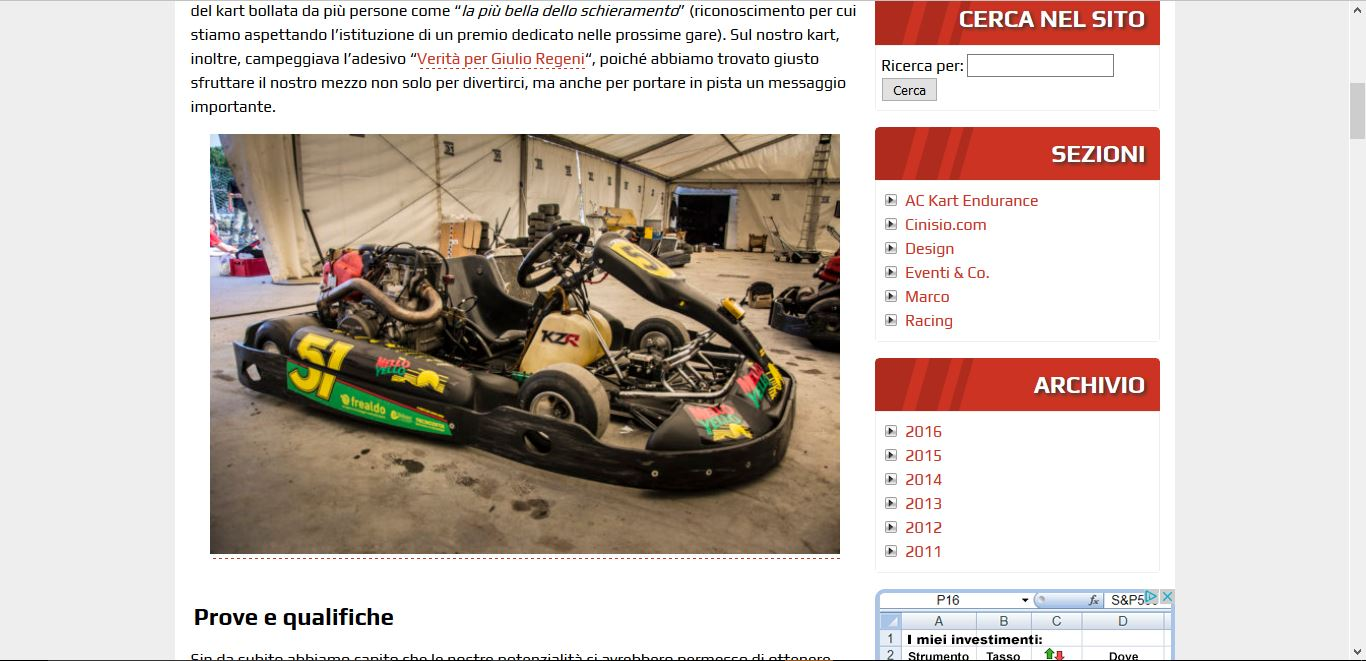
\includegraphics[width=\textwidth]{images/ImageBetweenText}
				\caption{Esempio di immagine che interrompe la lettura dell'articolo}
				\label{fig:ImageBetweenText}
			\end{figure}
			
	
	\newpage
	\subsection{Le immagini}
		Il sito presenta una grossa attenzione alle immagini alle quali sembra sia data più priorità rispetto al testo. Il numero di immagini in ogni pagina risulta molto elevato e spesso di troppo. Questo oltre ad occupare notevole spazio nella pagine con contenuto di poco interesse per l'utente medio comporta frustrazione, lo scanning iniziale della pagina(per esempio l'homepage), dato l'elevato numero di immagini, sarà quasi completamente bianco provocando disorientamento nell'utenza.
		
		A tal proposito si mostra nella figura \ref{fig:BlankHomepage1} la homepage completamente spoglia delle immagini, sicuramente il design si affievolisce ma questo si può considerare come quello che un utente visualizza nella fase dello scanning.
		
		\begin{figure} [h]
			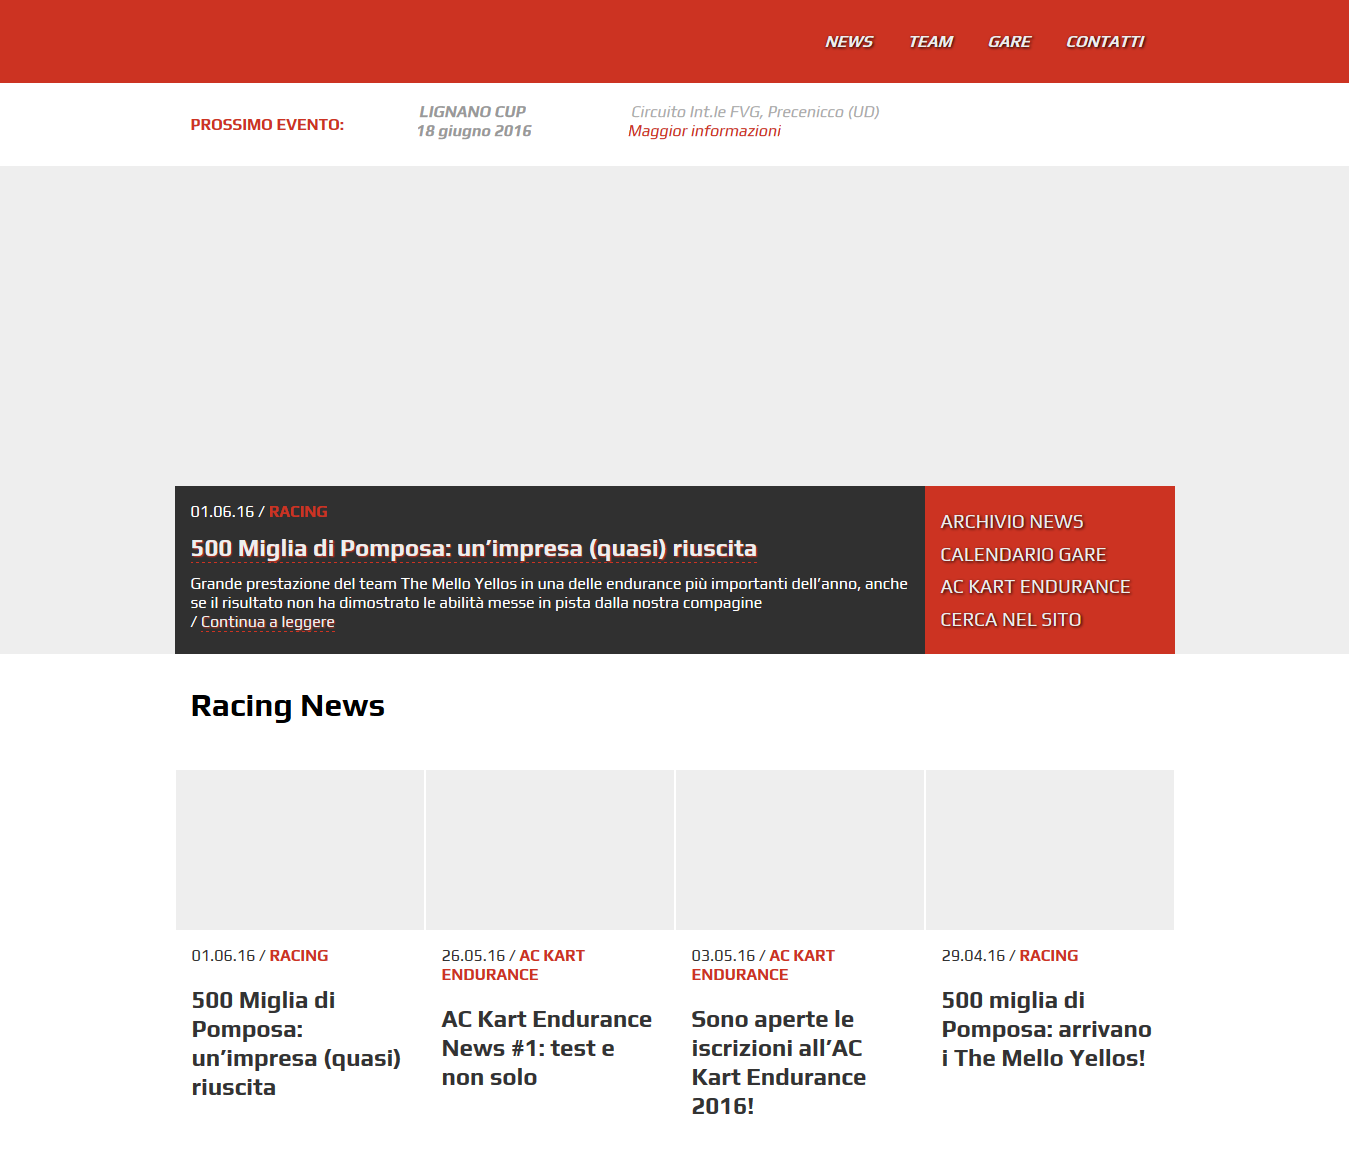
\includegraphics[width=\textwidth]{images/BlankHomepage1}
			\caption{La schermata iniziale della homepage priva di immagini}
			\label{fig:BlankHomepage1}
		\end{figure}
		
		%\begin{figure} [p]
			%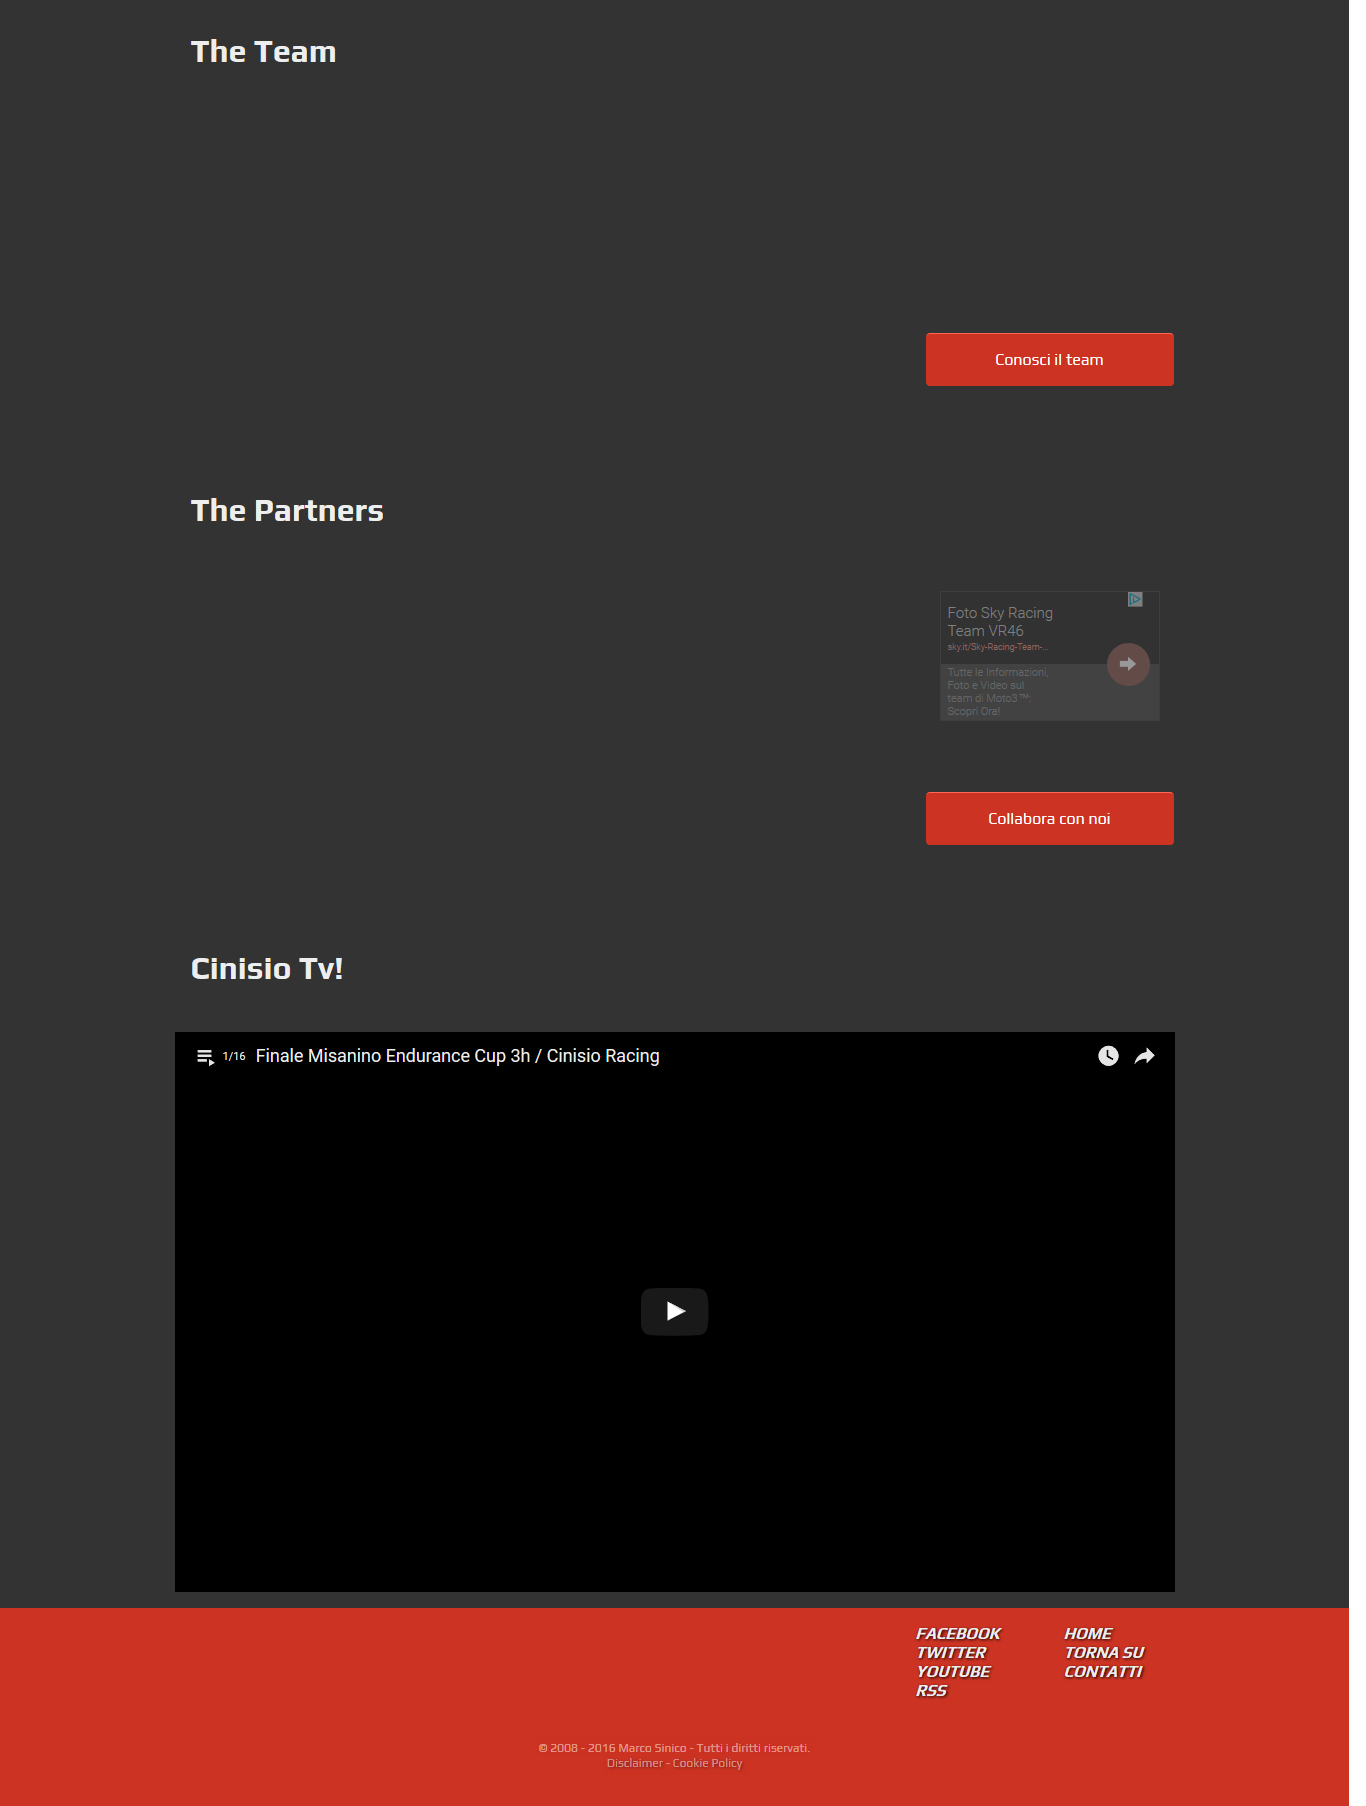
\includegraphics[width=\textwidth]{images/BlankHomepage2}
			%\caption{La homepage priva di immagini (parte 2)}
			%\label{fig:BlankHomepage2}
		%\end{figure}
		
		\newpage
		Da tale figura si può anche intuire quanto lo \textbf{scroll} sia in eccesso solo per dare spazio alle immagini. Il numero di parole all'interno nella pagina infatti è tale da poter essere incluso totalmente nella prima schermata eliminando quasi del tutto l'utilizzo dello scroll.
		
		Inoltre un altro grave riscontro sta nella non ``cliccabilità'' di alcune immagini. Prendendo sempre la homepage come riferimento, si evince che solo le immagini associate ad una new sono cliccabili, tutte le altre no: 
		\begin{itemize}
			\item Immagine a schermo intero delle ultime notizie;
			\item Le immagini del team;
			\item Le immagini che rappresentano gli sponsor.
		\end{itemize}
	
	In conclusione, un'enorme quantità di immagini con più importanza rispetto al testo. La maggioranza di esse non rappresentano link ipertestuali (click a vuoto dell'utente), appesantiscono la dimensione della pagina e sono causa di uno scroll elevato.
	
	\newpage
	\subsection{Cookie policy}
		Un punto a favore va alla gestione dell'avviso dei cookie, il banner di avviso è posizionato in basso alla pagina e non dà in alcun modo fastidio all'utente. Il pulsante per accettare e quindi nascondere l'avviso è bene in vista e facilmente cliccabile. Probabilmente si potrebbe aumentare le sue dimensioni per aumentare l'usabilità nell'impatto iniziale della prima visita.
		 
		\begin{figure} [h]
			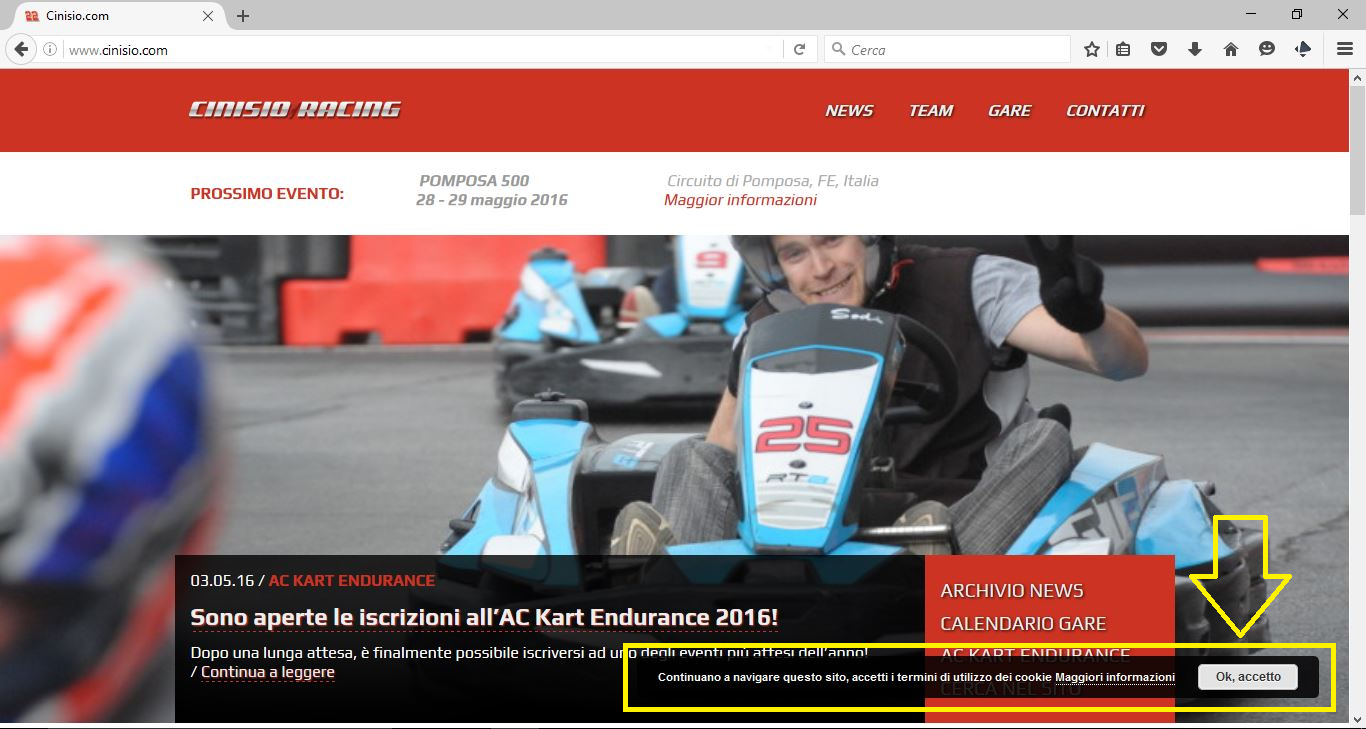
\includegraphics[width=\textwidth]{images/CookiePopUp}
			\caption{Il banner per accettare le policy dei cookie al primo accesso nella homepage}
			\label{fig:CookiePopUp}
		\end{figure}
		 	
	
	\newpage
	\subsection{Breadcrump}
		Il sito presenta un breadcrump solo per le pagine identificate come new o articoli. Il tipo di breadcrump utilizzato è quello ad \textbf{attributi}. Ad ogni new infatti gli viene associato un tag con la tematica che tratta.
		Nonostante questo sia molto utile per comprendere subito l'argomento trattato dall'articolo non soddisfa pienamente i canoni di usabilità. L'utente infatti non sa di essere nella sezione \textbf{news} poiché l'attributo mira solo a distinguere e a classificare le pagine new e non comprendono una visione più larga di tutto il sito.
		
	Risulta quindi necessario un semplice \textbf{location breadcrump} da affiancare agli attributi, purtroppo però questo c'è ma in una posizione errata e quindi invisibile per la maggioranza dell'utenza. Come mostrato in figura \ref{fig:LocationBreadcrump}, il location breadcrump è situato nel titolo della scheda, per cui, oltre ad essere in un luogo raramente consultato dall'utente, l'apertura di più schede comporta la perdita di questo sostituito dal browser con i tre puntini di sospensione (\dots).
		
		\begin{figure} [h]
			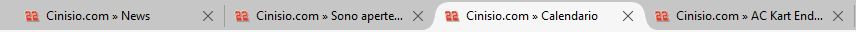
\includegraphics[width=\textwidth]{images/Dettaglio_PathInTheTitleCard}
			\caption{Il location breadcrump nel titolo della scheda}
			\label{fig:LocationBreadcrump}
		\end{figure}
		
		 In conclusione l'utente è privo di un breadcrump robusto su cui agganciarsi in caso di disorientamento. Il breadcrump ad attributi presente risulta insufficiente per la navigazione del sito e il location breadcrump anch'esso presente risulta inutilizzabile data la sua posizione scarsamente consultabile.
		 
	\newpage
	\subsection{Il footer}
		Una nota va fatta anche per la componente in basso ripetuta in tutte le pagine del sito: il footer. Nel sito in esame esso è composto da almeno due schermate di un normale schermo (figure \ref{fig:Footer1} e \ref{fig:Footer2}). Esso è composto dalle seguenti componenti:
		\begin{itemize}
			\item Racing news;
			\item The Team;
			\item The Parteners;
			\item Cinisio TV (solo homepage);
			\item Il footer vero e proprio.
		\end{itemize}
		
		\begin{figure} [h]
			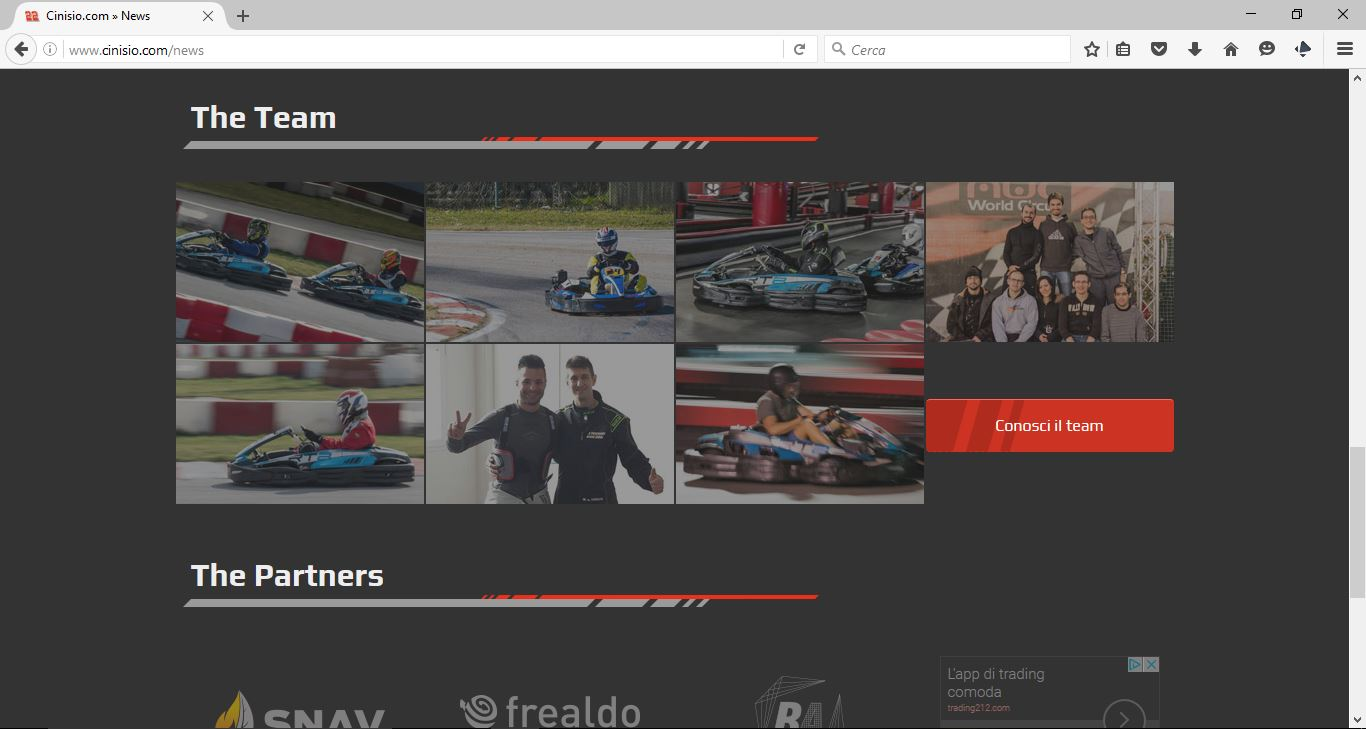
\includegraphics[width=\textwidth]{images/Footer_Part1}
			\caption{Parte 1 che compone il footer}
			\label{fig:Footer1}
		\end{figure}
		
		Per la parte \textbf{Racing new} troviamo due linee con layout a griglia delle ultime news pubblicate. Occupano troppo spazio della pagina (soprattutto negli articoli più lunghi), aumentano inutilmente lo scroll. Una linea di notizie può essere sufficiente anche se essa non dovrebbe essere ripetuta in tutte le pagine, soprattutto quelle degli articoli. Infatti qui è totalmente ridondante poiché esiste già un menu nel lato destro della pagine intitolato \textit{News recenti}
		
		Per quanto riguarda la parte \textbf{The Team} (figura \ref{fig:Footer1}) si può facilmente eliminare o sostituire, le immagini presentate appesantiscono la pagina, generano scroll e non sono cliccabili inoltre il pulsante corrisponde al link del menu se si clicca \textit{TEAM}.
		
		\begin{figure} [h]
			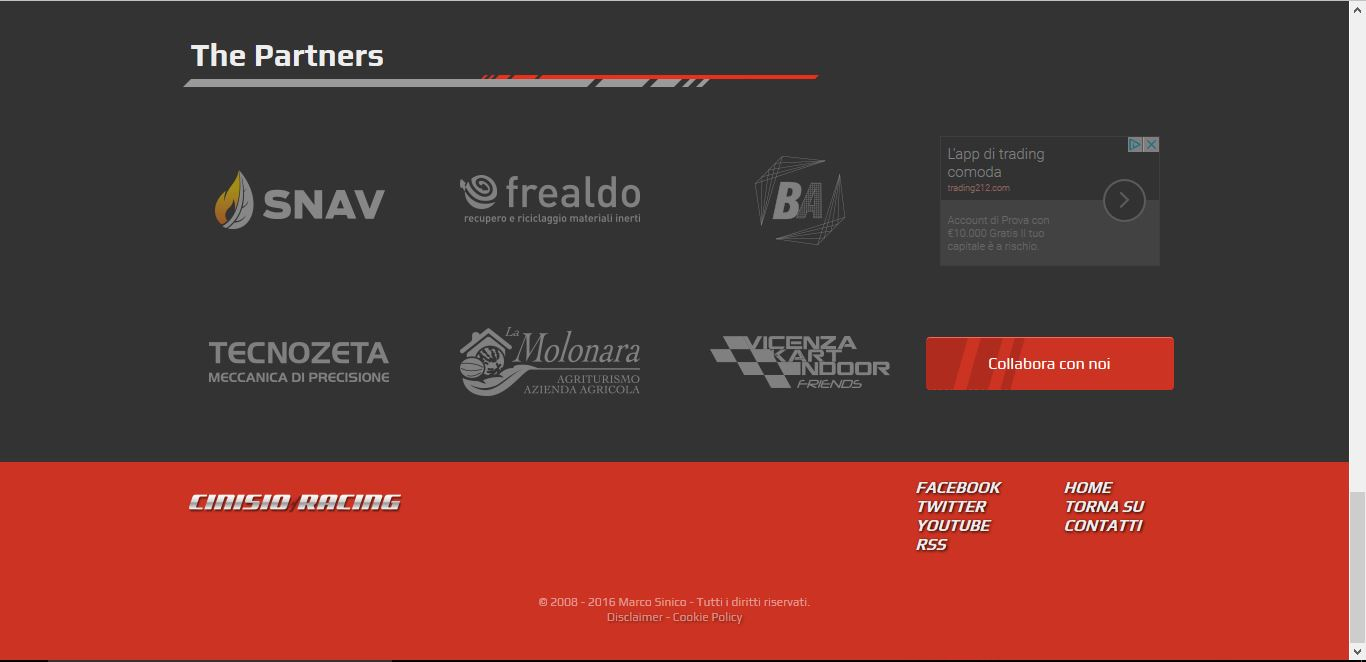
\includegraphics[width=\textwidth]{images/Footer_Part2}
			\caption{Parte 2 che compone il footer}
			\label{fig:Footer2}
		\end{figure}
				
		
		 La parte \textbf{The Partners} (figura \ref{fig:Footer2}) sebbene soffra del problema delle immagini non cliccabili si può accettare come posizionamento anche se con questa posizione nella pagina gli sponsor raramente saranno visti da un utente.	  		

		
		La parte \textbf{Cinisio TV}, disponibile solo nella homepage, invece meriterebbe una pagina dedicata, il player video streaming dal portale YouTube presenta buoni contenuti e funziona solo se richiesto (nessun avvio automatico). Spostarlo dalla homepage favorirebbe la fruizione dei video a tutti quegli utenti che non scrollano fino al footer della homepage e inoltre alleggerirebbe la homepage.
		
		Nell'ultima parte, che è il footer vero e proprio, si presentano i link ai vari social disponibili, stesso errore di prima, un utente non potrà mai usufruire di tali link perché troppo nascosti.
		
		\newpage
		\subsection{Metafore visive}
			Per metafora visiva si intende l'uso di effetti grafici che ingannano l'aspettativa dell'utente. Nel sito sono presenti varie metafore visive. Prima fra tutti quella delle \textbf{immagini} già precedentemente e più volte rimarcata. 
			
			Nella homepage solamente le immagini associate ad un articolo sono cliccabili e conducono l'utente alla pagina di quell'articolo, tutte le altre sono finti link. L'utente in questo caso è ingannato perché le immagini una volta posizionato il cursore su di esse si illuminano con un effetto simile a quello dei link. L'utente in questo caso sarà in condizione di \textit{gambling click} (ossia incerto nell'effetto del click) poiché non sa se tale click causerà uno zoom dell'immagine o l'apertura di una nuova pagina. Non solo, dei due effetti attesi nessuno si manifesterà (metafora visiva) infatti gli effetti del click saranno nulli.
			
			Seconda metafora visiva la troviamo nei \textbf{link}, essi non rispettano lo stile accettato comunemente nel web e lo ridefiniscono in modo complesso. L'utente non ha modo all'interno del sito di capire se un testo è un link e risulta difficile se non impossibile la comprensione di tale stile applicato, poiché cambia di pagina in pagina, infatti solo alcuni dei link già visitati cambiano opportunamente colore. Si sottolinea inoltre che tale errore di usabilità peggiora enormemente la fase di scanning.
			
			La terza e ultima metafora visiva è nelle \textbf{liste}, i classici punti neri affianco ad ogni elemento della lista sono sostituiti con ambigue icone del pulsante conosciuto come \textit{play}, per questo risulta un ottimo inganno per l'utente che si aspetta che tale icona sia cliccabile.
			
		\begin{figure} [h]
			\centering
			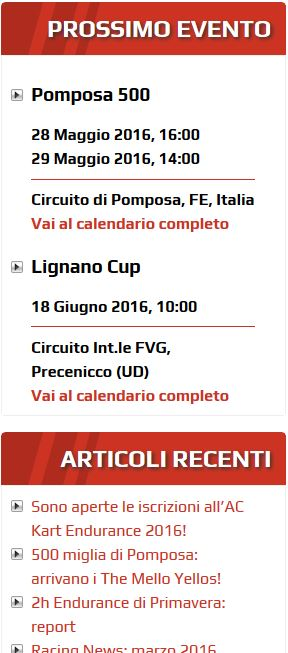
\includegraphics[scale=0.44]{images/MaybeImALink}
			\caption{L'icona ambigua non cliccabile delle liste - in questo caso accompagna dei titoli sopra e dei link cliccabili sotto}
			\label{fig:Footer2}
		\end{figure}
				


\section{Pubblicità}
	Il sito non presenta forme di pubblicità aggressiva (pop up o banner di grandi dimensioni) ma presenta solo dei piccoli banner classici di Google. Tuttavia a questi non gli è data importanza.
	
	\subsection{Banner}
	Nella homepage l'unico banner presente è situato nel pre-footer (figura \ref{fig:Homepage-Banner}) ed è sicuramente invisibile per la grande maggioranza dell'utenza.
	
	\begin{figure} [h]
		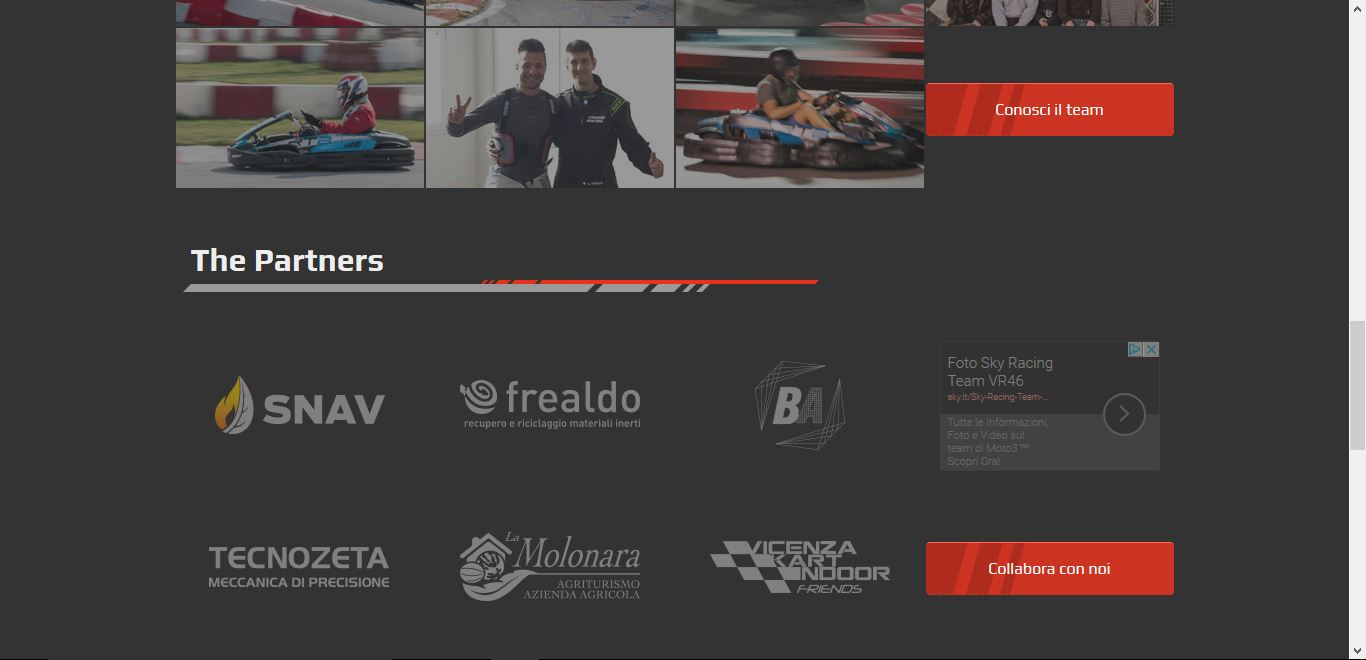
\includegraphics[width=\textwidth]{images/OpsABanner}
		\caption{L'unica pubblicità contenuta nella homepage}
		\label{fig:Homepage-Banner}
	\end{figure}
	
	In alcune pagine di new invece il banner entra in gioco ed è situato in primo piano a sinistra vicino al testo (figura \ref{fig:New-Banner}). Il posizionamento è azzeccato, non spezza il testo e non genera nessun fastidio per l'utente che può facilmente ignorarlo.
	
	
	In altre new e nelle altre pagine invece il banner è ancora messo in secondo piano, questa volta nella parte laterale destra in basso del sito. Anche qui è raro che un utente lo possa visualizzare.
	
	\subsection{Conclusioni}
		Da quanto visualizzato il sito non utilizza propriamente la pubblicità e dimostra quindi di non avere nessuno scopo di lucro. I posizionamenti anche se controproducenti per l'idea di banner non si sovrappongono mai all'usabilità del sito che rimane intatta.
	
	\begin{figure} [h]
		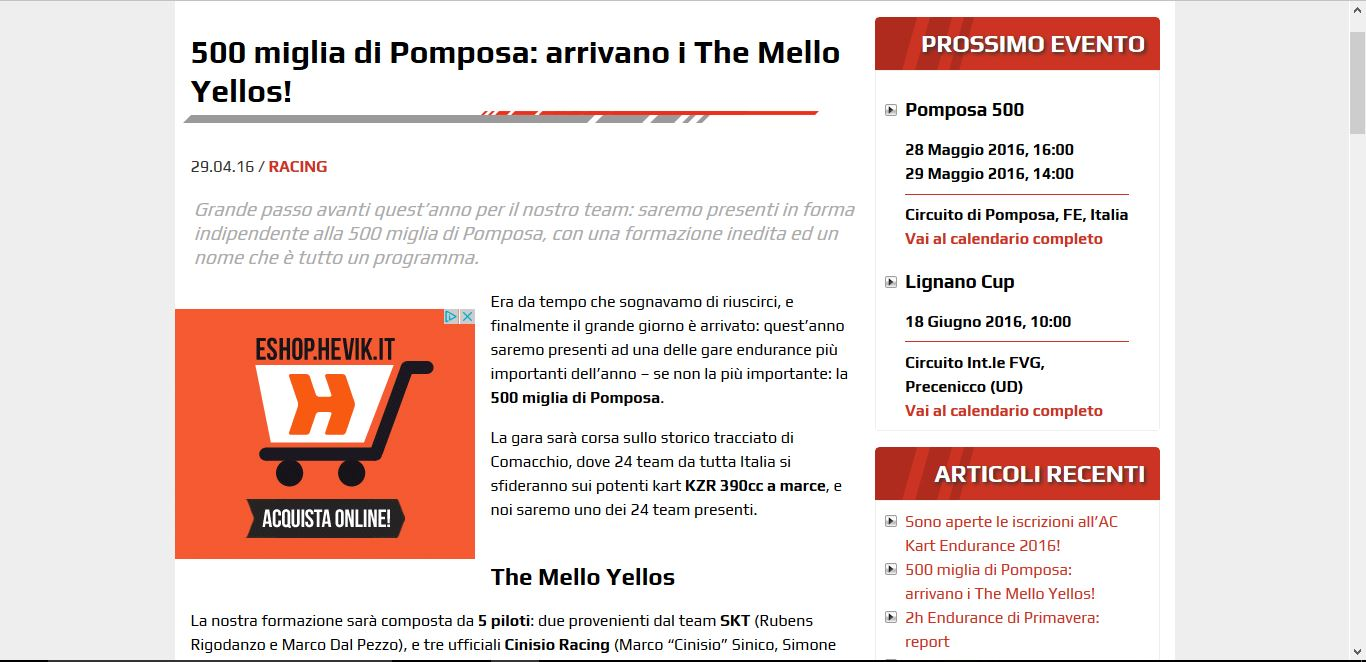
\includegraphics[width=\textwidth]{images/OpsABannerInANew}
		\caption{Posizione del banner in alcune pagine news}
		\label{fig:New-Banner}
	\end{figure}	
	
	\begin{figure} [h]
		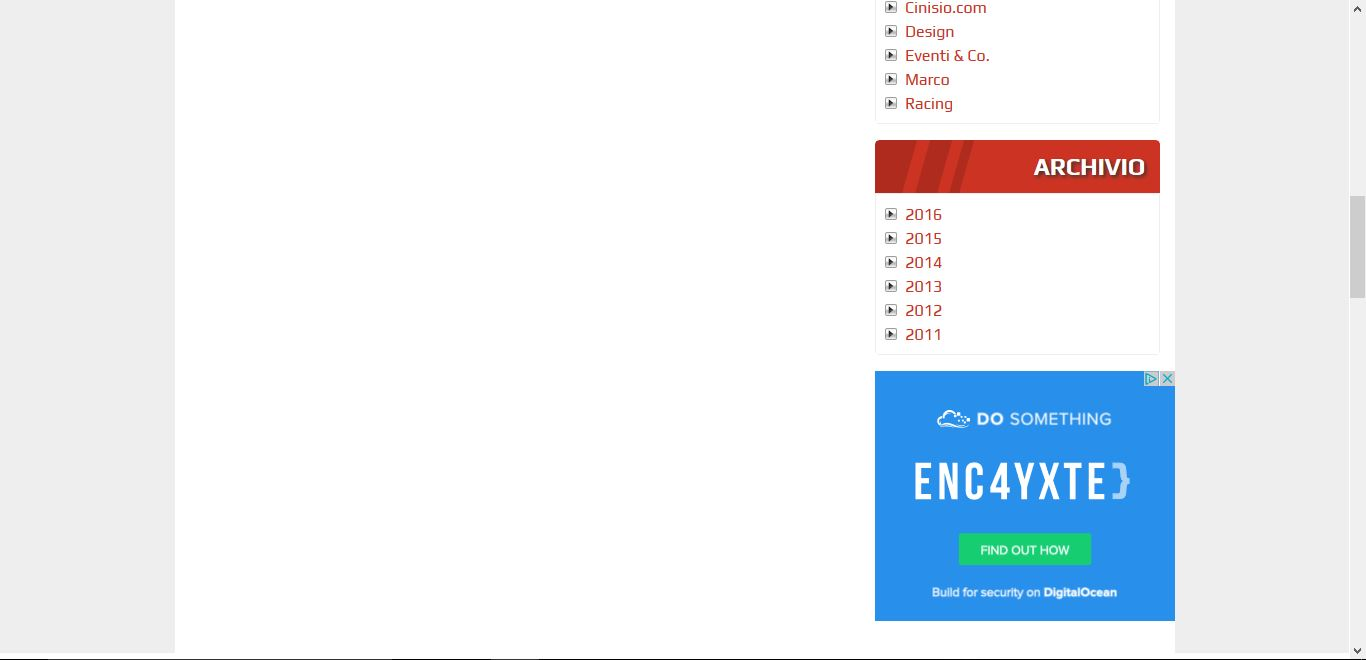
\includegraphics[width=\textwidth]{images/OpsAnotherBanner}
		\caption{Posizione alternativa del banner in altre pagine del sito}
		\label{fig:AnotherBanner}
	\end{figure}


\section{La ricerca}
	In base al numero di pagine la funzionalità di ricerca diventa fondamentale in un sito internet. Nel caso di cinisio.com dalle analisi fatte con strumenti online le pagine risultato essere \textbf{quasi 300} (figura \ref{fig:NumeroDiPagine}).
	
	
	\begin{figure} [h]
		\centering
		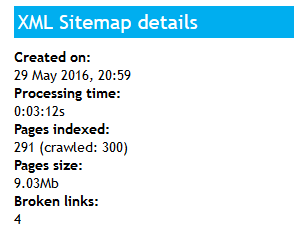
\includegraphics[width=0.5\textwidth]{images/NumeroDiPagine}
		\caption{Numero di pagine dopo l'analisi con il tool \textit{XML Sitemap}}
		\label{fig:NumeroDiPagine}
	\end{figure}
	
	In tal caso è necessario dotare il sito di una funzionalità di ricerca ma questa non c'è. Infatti nella homepage non troviamo nessuna casella di ricerca (search box) e solo dopo aver controllato attentamente si trova il link ad una presunta ricerca nella didascalia dell'immagine in primo piano (figura \ref{fig:Homepage-Ricerca}).
	
	\begin{figure} [h]
		\centering
		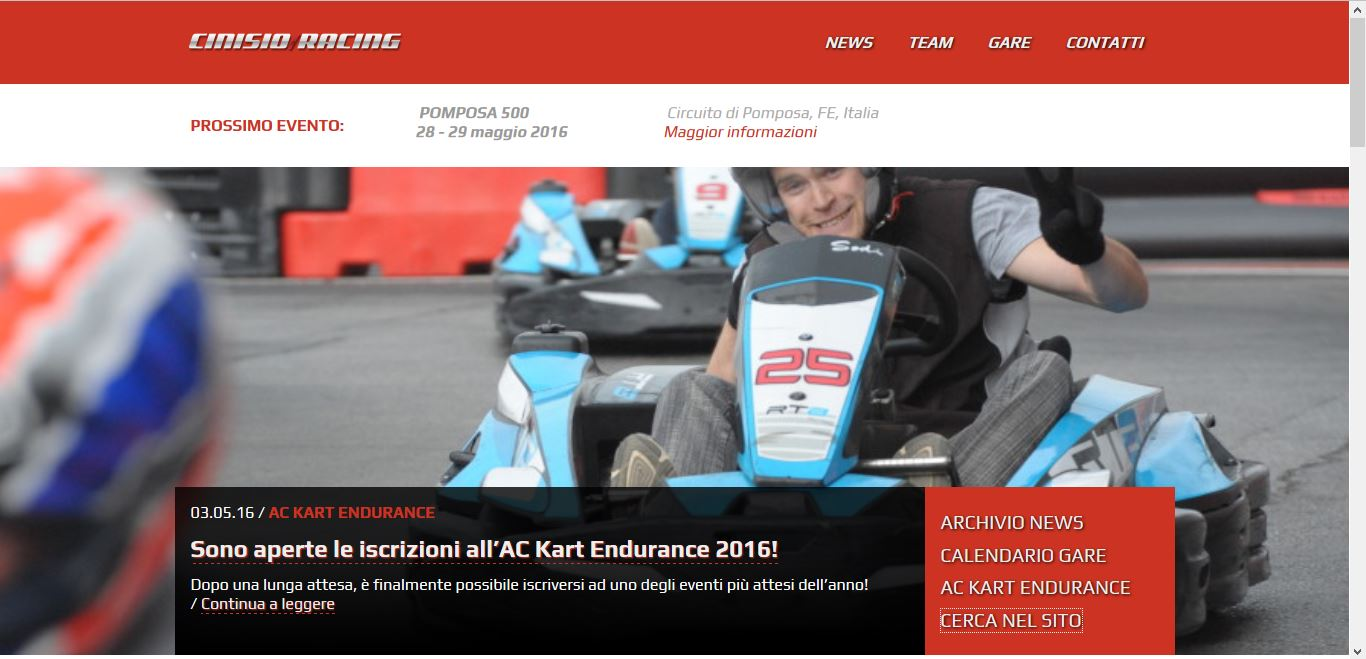
\includegraphics[width=\textwidth]{images/SearchOption_WhereItIs}
		\caption{Il link per la ricerca nel sito}
		\label{fig:Homepage-Ricerca}
	\end{figure}
	
	Il link però porta alla pagina con il messaggio in figura \ref{fig:RicercaNonDisponibile} e subito dopo aver descritto che la funzionalità non è implementata nel sito incoraggia l'utente ad utilizzare un search box a lato nella pagina. 
	
	\begin{figure} [h]
		\centering
		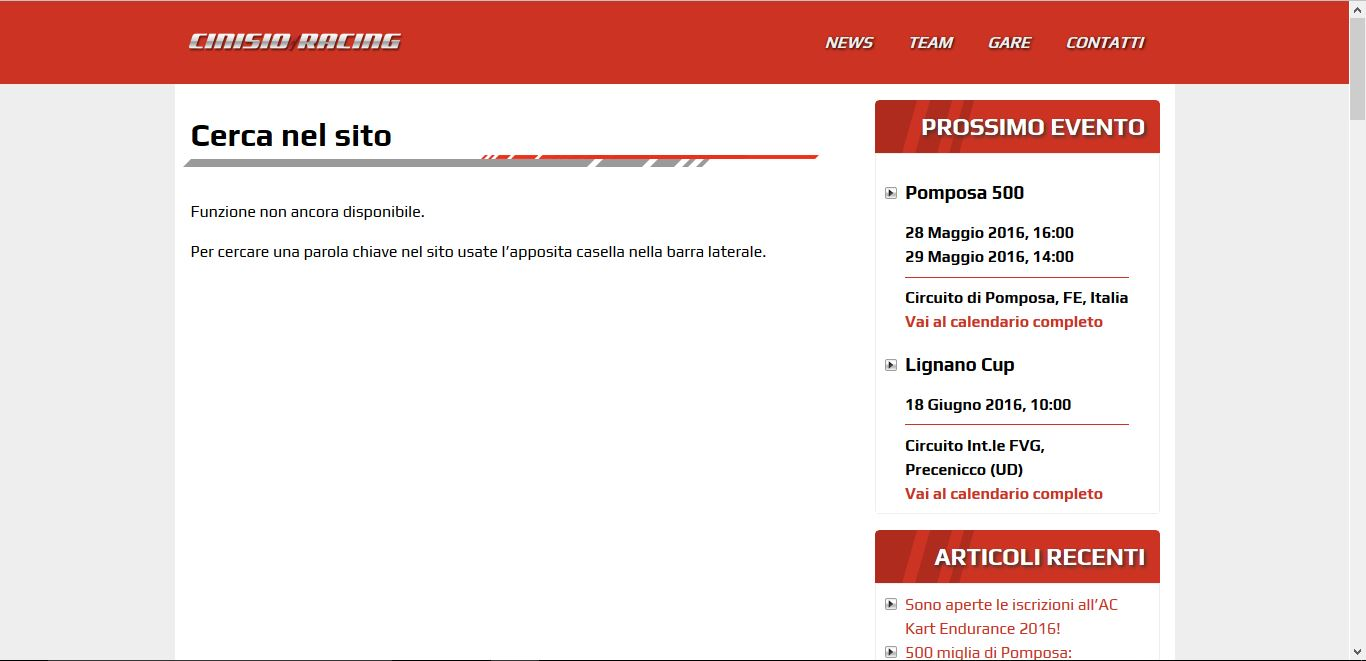
\includegraphics[width=\textwidth]{images/PoorSearchBox}
		\caption{L'avviso contraddittorio il quale dice che la funzionalità di ricerca nel sito non è presente ma è disponibile a lato}
		\label{fig:RicercaNonDisponibile}
	\end{figure}
	
	L'utente così paziente da leggere anche la seconda riga dell'avviso si accorgerà quindi che effettivamente esiste un search box situato a lato dopo uno scroll e solo in alcune pagine del sito (figura \ref{fig:RicercaSearchBox}). La posizione nascosta sembra intenzionale per scoraggiarne l'uso -- oltre a scoraggiare il proseguimento della navigazione nel sito -- ma alcune prove effettuate con la search box trovata rivelano che la funzionalità di ricerca c'è e funziona abbastanza bene. Dalla figura \ref{fig:RicercaRisultati} possiamo vedere come una semplice ricerca con le keyword \textit{Kart} e \textit{endurance} hanno prodotto una lista di risultati coerente con le attese.
	
	\begin{figure} [h]
		\centering
		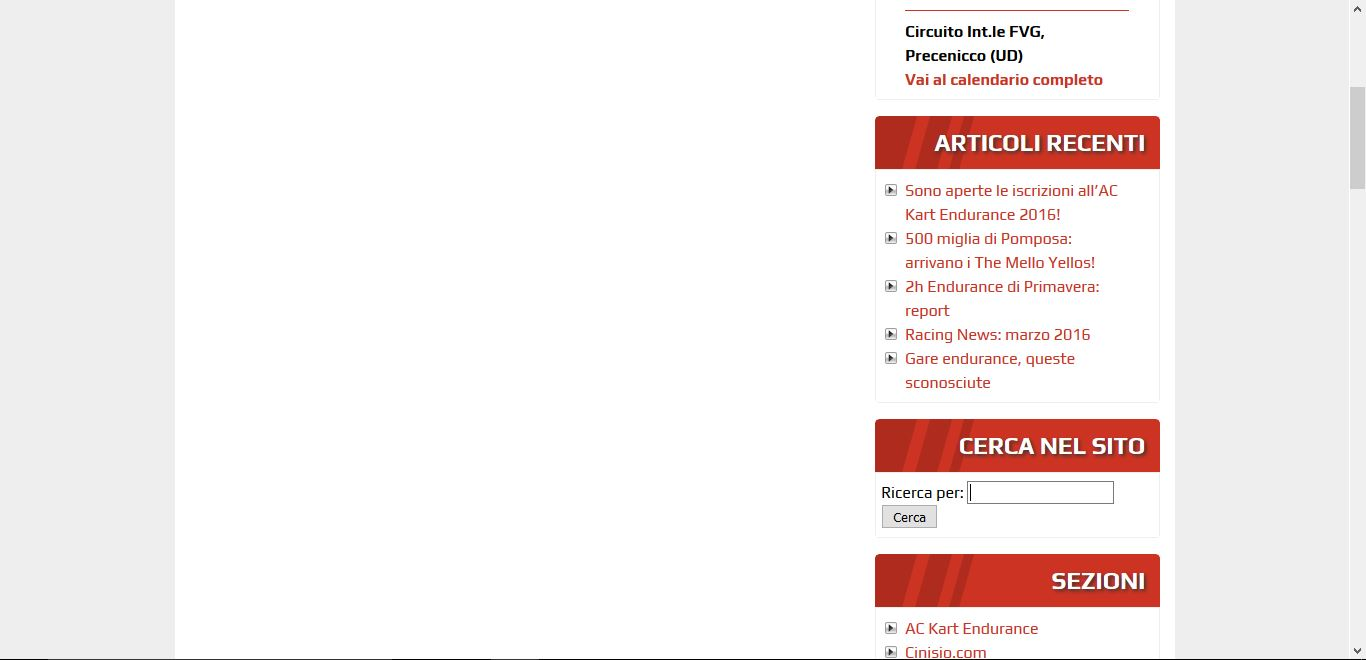
\includegraphics[width=\textwidth]{images/FinallyTheSearchBox}
		\caption{La posizione del search box in alcune pagine del sito}
		\label{fig:RicercaSearchBox}
	\end{figure}
	
	\begin{figure} [h]
		\centering
		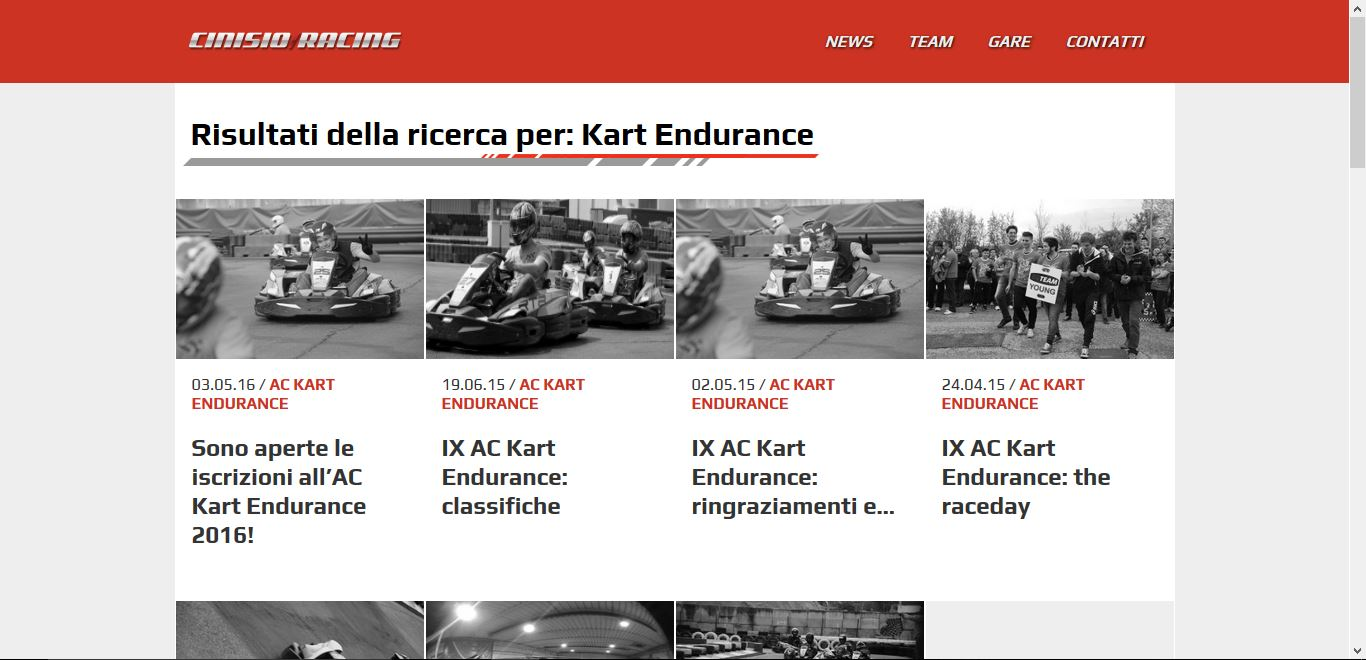
\includegraphics[width=\textwidth]{images/SearchResult}
		\caption{I risultati della ricerca delle keyword \textit{Kart Endurance}}
		\label{fig:RicercaRisultati}
	\end{figure}
	
	Per un tecnico della materia è evidente che nel sito sono presenti due ricerche differenti: una molto più raffinata ma non implementata e una più imprecisa ma già implementata. Il problema è che il passaggio da una all'altra deve essere fatto senza lasciare l'utente disorientato con un messaggio d'avviso contraddittorio. 
	La search box deve essere messa bene in vista, anche nella homepage, non importa se non porta a risultati precisi, all'utente deve essere data l'opportunità di ricercare all'interno di un sito composto da quasi 300 pagine.


\section{Usabilità su mobile}
	Poiché oggi la maggioranza dell'utenza naviga con dispositivi mobili questa sezione è d'obbligo. 
	In ambito mobile i problemi di usabilità prima affrontati si amplificano, per motivi di sintesi quindi si è analizzato la \textbf{mobile responsiveness} e i \textbf{tempi di caricamento}, caratteristiche che ritengo essenziali per l'usabilità in ambiente mobile.

	\subsection{Responsiveness}
		Il layout del sito degrada elegantemente e si nota lo sforzo attuato per garantire una gradevole navigazione su mobile senza sacrificare il layout. Sottoporre la homepage al test dello strumento online di Google \href{https://www.google.com/webmasters/tools/mobile-friendly/?hl=it}{Mobile Friendly} fa guadagnare il massimo punteggio, ogni accortezza proposta da Google è implementata.
		
	\subsection{Tempi di caricamento}
		Molto male invece nei tempi di caricamento, lo strumento \href{https://developers.google.com/speed/pagespeed/insights/}{SpeedTest} assegna un punteggio di 37 punti su 100. 
		
		I tempi di caricamento della sola homepage usufruendo di una connessione wi-fi con uno smartphone di fascia bassa misurano più di 10 secondi, ulteriori test con telefoni più prestanti e sempre con connessione wi-fi misurano quasi 10 secondi. Un'enormità se consideriamo che l'utente medio concede solo 2 secondi di attesa.
		
		La causa di questo possiamo individuarla nella dimensione della pagina:
		La homepage pesa più di 3 MB come mostra la figura (figura \ref{fig:PerformanceEmptyCache}) e il caching non garantisce un risparmio significativo (figura \ref{fig:PerformanceWithCache}). Il sito in generale contiene troppo codice Javascript e troppe immagini non compresse e nella maggior parte dei casi di troppo. Alcuni possibili rimedi immediati sono:
		\begin{itemize}
			\item delegare il download delle librerie Javascript a server più prestanti in modo da alleggerire le trasmissioni dal sito e velocizzare i tempi di download;
			\item comprimere le immagini o meglio ridurne la presenza in tutte le pagine del sito;
			\item comprimere tutti i file scaricati alla visita di una pagina (CSS, JAvascript ecc.), sfruttando strumenti che eliminano gli spazi inutili per esempio;
			\item raggruppare tutti i file scaricati alla visita di una pagina in un unico file così da evitare continue richieste client-server.
		\end{itemize}
		
		\begin{figure}
			\centering
			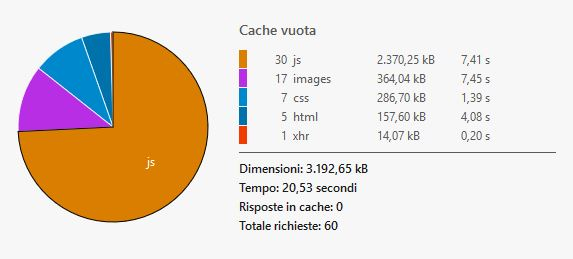
\includegraphics[scale=0.8]{images/PerformanceEmptyCache}
			\caption{Dimensione file di download per la homepage}
			\label{fig:PerformanceEmptyCache}
		\end{figure}		
		
		\begin{figure}
			\centering
			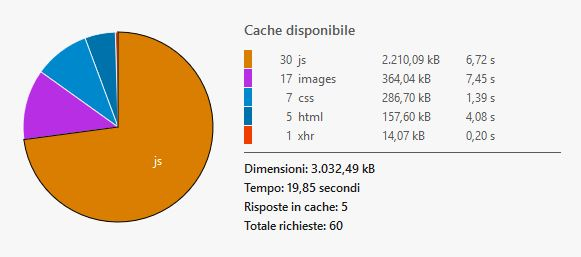
\includegraphics[scale=0.8]{images/PerformanceWithCache}
			\caption{Dimensione file di download per la homepage con l'uso della cache}
			\label{fig:PerformanceWithCache}
		\end{figure}


\section{Conclusioni}

	\begin{table}
		\centering
		\begin{tabular}[width=\textwidth]{lcc}
			\toprule
			\textbf{Tematica} & \textbf{Note} & \textbf{Voto} \\
			\toprule
			
			Navigabilità & \dots & ? \\
			\midrule
			Contenuto & & ? \\
			\midrule
			Pubblicità & & \\
			\midrule
			Ricerca & & \\
			\midrule
			Responsiveness & & \\
			\midrule
			\textbf{Voto totale} & & \textbf{?} \\	
			\bottomrule
			
		\end{tabular}
		\caption{Conclusioni}
		\label{tab:Conclusioni}
	\end{table}

\end{document}	